%
% VBrowser
%

\chapter{Customization}
\label{chap:customization}

\section{Custom viewers/plugins}

The VBrowser supports two kind of extension or plugins. One is for protocol 
implementations or 'VDrivers', The other are VBrowser Viewer extensions or Viewer 
plugins. The first are mapped to URI schemes like 'srm://' the latter are mapped to 
resource mimetypes like 'text/plain'. \\
\par
You can install extra viewers or VBrowser plugins in the following directories 
(create them if they don't exist):

\begin{itemize}
  \item \Path{VLETINSTALL/lib/plugins}: for installation plugins.
    \item \Path{HOME/.vletrc/plugins}: path for user plugins.
\end{itemize}

A \vbrowser\ plugin can be a single jar file or a directory that contains the needed
jar file and (optional) used libraries. The filename or directory must 
be the full classname of the plugin. 
This name triggers the VBrowser upon startup to load the plugin. 
For example the custom VTK image viewer which can be install at one of the
following locations:\\
\\
\tab \Path{VLETINSTALL/lib/plugins/nl.uva.vle.app.vtk.viewer.NiiViewer/}\\
\\	
for system wide installation of custom plugins, or:\\
\\
\tab \Path{HOME/.vletrc/plugins/nl.uva.vle.app.vtk.viewer.NiiViewer/}\\
\\
for custom plugins installed for a single user only (in his or hers HOME directory). \\
\\
Some viewers might need extra configuration. For example in the case of
the above VTK viewer, specifying the VTK library paths as follows:\\
\\
\tab \Code{export LD\_LIBRARY\_PATH=\$LD\_LIBARY\_PATH:/opt/vl-e/vtk\_5.0.2/lib:/opt/vl-e/mesa3d\_6.4.2/lib}\\
\\
The above library paths are the installation paths as specified on the VL-e PoC
environment (R2). You can add them to your \Path{.bashrc} or add them to the
installation configuration in \Path{VLET\_INSTALL/etc/vletenv.sh} if library
paths are not already setup as specified. \\
\\
Extra plugins can be downloaded from the VL-e gforge 
site: \Link{gforge.vl-e.nl/frs/?group\_id=19}

\section{Custom Mimetypes and icons}

Mimetypes are a way of telling an application what kind of content is in the
file or resource. In most cases this is a simple mapping of an extension to a 
standard defined mimetype. This mimetype is a simple string which describes 
the type of content, for example ``text/plain'' or ``image/jpeg''. Usually it
consists of a generic part (``text/'' or ``image/'') and a specific part
(``plain'' or ``jpeg'') seperated by a (forward) slash.\\ 
The following files defines the mimetypes used in \VLET:

\begin{itemize}
  \item \Path{VLETINSTALL/etc/mime.types}: for installation configured mime
  types.
  \item \Path{HOME/.vletrc/mime.types}: for user configured mime types.
\end{itemize}

The syntax of the mimetype configuration is the mimetype name followed by a list
of extensions or complete filename(s) as follows: \\
\\
\tab \Variable{type/subtype EXT1 EXT2 EXT3\ldots}\\
\\
An example of some standard mimetypes is given as follows. First the
mimetype name is given followed by their extension(s):\\
\\
\begin{boxedlisting}[170]
\begin{verbatim}
###
# File    : mime.types
# Location: $VLET_INSTALL/etc/mime.types
# ---
# Default mime types:  <MIMETYPE>  <EXTENSION1> <EXTENSION2> ...
#

image/x-xbitmap                 xbm 
image/x-xpixmap                 xpm
image/jpeg                      jpeg jpg jpe JPG
text/rtf                        rtf
text/plain                      txt
# some custom mimetypes examples: 
application/jglite-jobids       vljids 
application/taverna-scuffle     scuffle
application/feat-fsf            fsf FSF 

#end default mime types file 
\end{verbatim}
\end{boxedlisting}

\subsection{User defined mimetypes}

A user can override the default mimetype for a resource or specify a new one  
by adding a line in the \Path{HOME/.vletrc/mime.types} file (if the file is not there the user can created) as follows:\\
\\
\begin{boxedlisting}
\begin{verbatim}
##
# File    : mime.types 
# Location: $HOME/.vletrc/mime.types
# ---
# User defined mime types 

# customized mime type for VL-e Text: 
application/vle-text      vletxt txt TXT inf info

# end user defined mime types
\end{verbatim}
\end{boxedlisting}\\
\\
Now .txt (and .TXT, .inf, .info) files will have the "application/vle-text" mimetype 
as can be seen in Figure:\ref{fig:custom_mimetypes}\\
\\
\begin{figure}[htbp]
\centerline{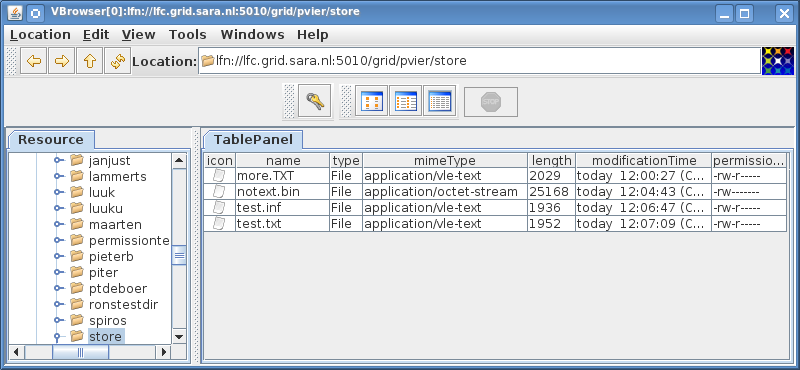
\includegraphics[scale=0.5]{vbrowser_mimetypes}}
\caption{Custom Mimetypes}
\label{fig:custom_mimetypes}
\end{figure}\\
\\
\\
\subsection{Web server mimetypes}

When browsing websites and viewing resources at web servers, the web server has the 
responsibility to return the correct mimetype for the viewed resource. 
For example an html file has the mimetype "text/html" but the URL might not always 
point to a location which ends with '.html'.
Also a query or server side script (php) might return content which differs from what 
might be expected when inspecting the URL, which for example might end in ".php". 
Configuring a web server to return custom mimetypes can be done in different ways and
is highly dependant on the used web server and (Linux) environment it runs in.\\
\\
Below configuration files for a Linux+Apache 2.0 setup: 
\begin{itemize}
  \item \Path{/etc/mime.types} Global system (Linux) mime.types file.   
  \item \Path{/etc/httpd/conf/httpd.conf} Custom HTTPD configuration file or:  
  \item \Path{/etc/apache2/httpd.conf} Custom apache 2.0 configuration file. 
\end{itemize}
 
The \Path{/etc/mime.types} follows the same syntax as described in the previous paragraph.
Changing this file will change global settings for the whole (Linux) system.\\  
\\
Below an example of extra configuration settings which can be added to the \Path{httpd.conf} file.
The location of this file depends on used web server and Linux distribution. 
See the documentation of the used web server for the correct location of this file.\\
For example, add the following custom mimetypes to the \Path{httpd.conf} file
to allow (glite) job monitoring resources to have the correct mimetype:\\
 
\begin{boxedlisting}
\begin{verbatim}
###
# Add custom VBrowser mime types. 
# Add glite jobids: 
AddType application/glite-jobids .vljids
# Add job output files ".out" and ".err" as plain text:  
AddType text/plain .out
AddType text/plain .err
\end{verbatim}
\end{boxedlisting}

After changing this file the web server needs to be restarted for the changes to have effect. 
\\ 
\\
\subsection{Magic types}
Another way to determine the file content is by matching the first bytes of a
resource with well known 'magic types' which specify the type of file. 
For example Linux executables have the letters 'ELF' in the beginning of 
the file which specifies it is an Linux Executable. \\
Other examples are: GIF files (.gif) start with the ASCII letters 'GIF' and 
WAV files (.wav) start with the letters 'RIFF' and have the letter 'WAVE' in the
RIFF header.
\\ Magic types are not supported (yet) by the VBrowser but are available in 
the \VLET\ Java API through the MimeTypes class 
(\Class{nl.uva.vlet.util.MimeTypes})
and can be used by, for example, plugins to further determine the (actual) file
contents. 

\subsection{Custom icons}

Each resource which has a mimetype is mapped to a (default) icon based 
on the mimetype. The name of the icon is the mimetype with forbidden
characters (like a forward slash) substituted with a dash (``-'') and the
extension ``.png'' is added.
For example the mimetype:``application/vle-text'' is transformed to the icon 
name:``application-vle-text.png''\\
\\
If this icon exists in either the installation directory for mimetype icons or the
user directory for mimetype icons, this icon will be used. 
To add mimetype icons, add the icon to one of the following directories:\\
\\ 
\tab \Path{HOME/.vletrc/icons/mimetypes}\\
\\ 
Use the above location for user configured icons. To make the icons
available for all users, use the installation directory below:\\
\\
\tab \Path{VLET\_INSTALL/lib/icons/mimetypes}\\
\\
In the example of the custom mimetype ``application/vle-text'' you can create
a customized icon named:``application-vle-text.png" which should have the
following path:\\ \\
\tab \Path{HOME/.vletrc/icons/mimetypes/application-vle-text.png}\\
\\
All text files will now have the customized 'vle' icon as can be seen 
in Figure \ref{fig:custom_icons}\\
\\
\begin{figure}[htbp]
\centerline{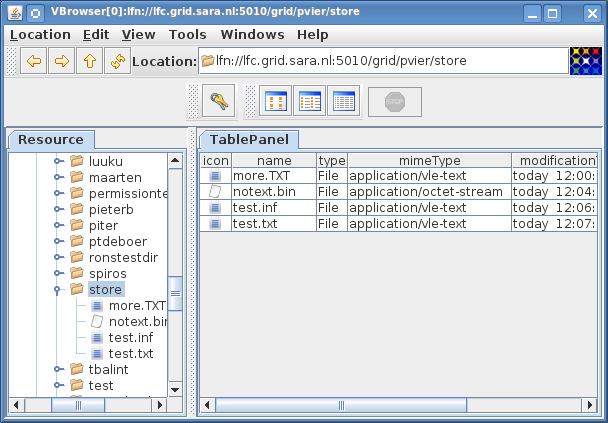
\includegraphics[scale=0.5]{vbrowser_custom_icons}}
\caption{Custom Icons}
\label{fig:custom_icons}
\end{figure}\\
\\
You can also put the icon in your installation by creating it at the following
path:\\
\\
\tab \Path{VLET\_INSTALL/lib/icons/mimetypes/application-vle-text.png}\\

\subsection{Viewer preferences and defaults}

To specify which viewer (vbrowser plugin) is used the user can configure the file
\Path{HOME/.vletrc/viewerconf.prop}.
This file specifies per line the mimetype and the viewerclass which is started
as default viewer when the user opens or clicks (on) a resource.
The syntax is as follows:\\
\\
\tab \Code{mimetype/mimesubtype=viewerclass}\\
\\
For example to specify a new viewer for the ``application/vle-text'' mimetype,
add a line as follows:\\

\begin{boxedlisting}
\begin{verbatim}
##
# File    : viewerconf.prop 
# Location: $HOME/.vletrc/viewerconf.prop
#---
# Mimetype/viewer class mapping file 
# <MIMETYPE>=<VIEWERCLASS> 

# viewerclass mapping for the application/vle-text mimetype:
application/vle-text=nl.uva.vlet.gui.viewers.HexViewer

# end viewerconf.prop file 
\end{verbatim}
\end{boxedlisting}\\
\\
Now, instead of the default textviewer, the actual bytes will be shown in the 
HexViewer utility.\\
Other default vbrowser internal viewer classes are:
\begin{verbatim}
	nl.uva.vlet.gui.viewers.TextViewer
	nl.uva.vlet.gui.viewers.HexViewer 
	nl.uva.vlet.gui.viewers.VHTMLViewer
	nl.uva.vlet.gui.viewers.ImageViewer
\end{verbatim}

For information about how to create custom plugins, see the VLET Developers 
Guide (ref:[]).


 